\documentclass[english,11pt]{amsart}
\usepackage[latin9]{inputenc}
\usepackage{amsmath}
\usepackage{amssymb}
\usepackage[backref=page,colorlinks,citecolor=blue,bookmarks=true]{hyperref}\hypersetup{linkcolor=blue,  citecolor=blue, urlcolor=blue}
\usepackage{tikz}
\usetikzlibrary{cd}
\usetikzlibrary{shapes}
\usepackage[backref=page,colorlinks,citecolor=blue,bookmarks=true]{hyperref}\hypersetup{linkcolor=blue,  citecolor=blue, urlcolor=blue}

\begin{document}

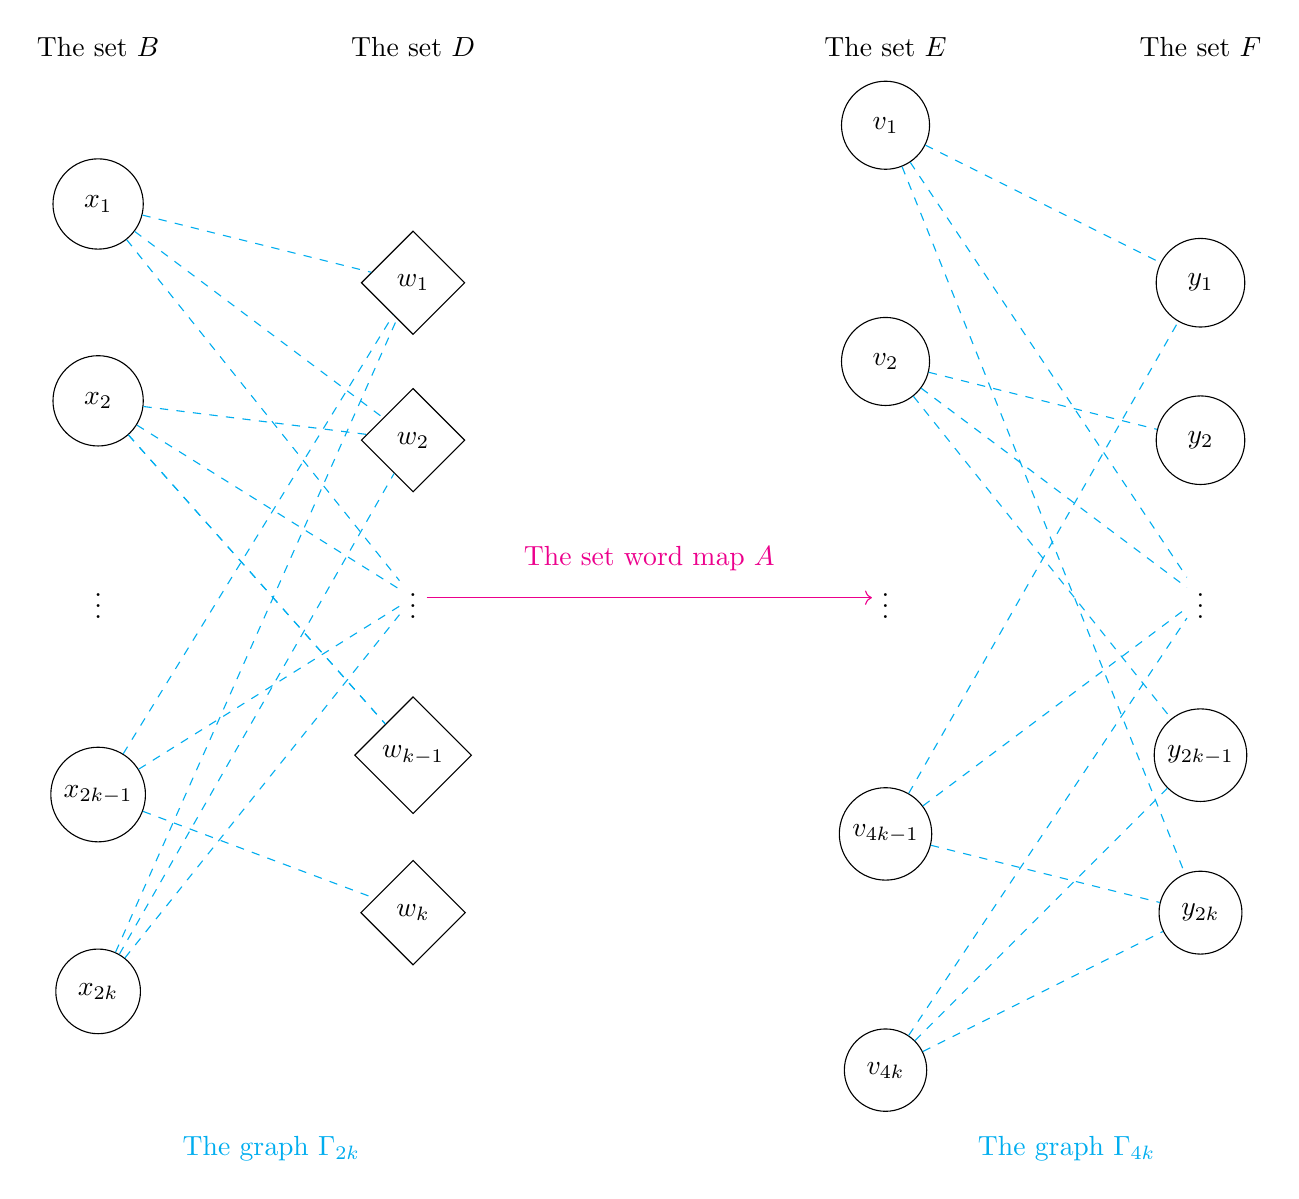
\begin{tikzpicture}[scale=1]
\node[color=black] (B) at (-1,7) {The set $B$};
\node[color=black] (D) at (3,7) {The set $D$};

\node[color=black] (E) at (9,7) {The set $E$};

\node[color=black] (F) at (13,7) {The set $F$};



\node[draw, color=black, shape=circle] (x1) at (-1,5) { $\ \ x_{1}\ \ $};

\node[draw, color=black, shape=circle] (x2) at (-1,2.5) { $\ \ x_2\ \ $};

\node (xdots) at (-1,0) { $\vdots$};

\node[draw, color=black, shape=circle] (x2k-1) at (-1,-2.5) { $x_{2k-1}$};

\node[draw, color=black, shape=circle] (x2k) at (-1,-5) { $\ x_{2k}\ $};


\node[draw, color=black, shape=diamond] (w1) at (3,4) { $\ w_1\ $};

\node[draw, color=black, shape=diamond] (w2) at (3,2) { $\ w_2\ $};

\node (wdots) at (3,0) { $\vdots$};
\node[draw, color=black, shape=diamond] (wk-1) at (3,-2) { $w_{k-1}$};
\node[draw, color=black, shape=diamond] (wk) at (3,-4) { $\ w_{k}\ $};


\node[color=cyan] (graph2k) at (1.2,-7) { The graph $\Gamma_{2k}$};


\node[draw, color=black, shape=circle] (v1) at (9,6) { $\ \ v_1\ \ $};

\node[draw, color=black, shape=circle] (v2) at (9,3) { $\ \ v_2\ \ $};

\node (vdots) at (9,0) { $\vdots$};
\node[draw, color=black, shape=circle] (v4k-1) at (9,-3) { $v_{4k-1}$};
\node[draw, color=black, shape=circle] (v4k) at (9,-6) { $\ v_{4k}\ $};

\node[color=magenta] (Awordmap) at (6,0.5) { The set word map $A$};


\node[draw, color=black, shape=circle] (y1) at (13,4) { $\ \ y_1\ \ $};

\node[draw, color=black, shape=circle] (y2) at (13,2) { $\ \ y_2\ \ $};

\node (ydots) at (13,0) { $\vdots$};

\node[draw, color=black, shape=circle] (y2k-1) at (13,-2) { $y_{2k-1}$};

\node[draw, color=black, shape=circle] (y2k) at (13,-4) { $\ y_{2k}\ $};
\node[color=cyan] (graph4k) at (11.3,-7) { The graph $\Gamma_{4k}$};


%edges pauli X
\draw[cyan, -, dashed] (x1)--(w2);
\draw[cyan, -, dashed] (x2)--(wk-1);
\draw[cyan, -, dashed] (x1)--(wdots);
\draw[cyan, -, dashed] (x1)--(w1);
\draw[cyan, -, dashed] (x2)--(wk-1);
\draw[cyan, -, dashed] (x2)--(w2);
\draw[cyan, -, dashed] (x2)--(wdots);
\draw[cyan, -, dashed] (x2k-1)--(wdots);
\draw[cyan, -, dashed] (x2k-1)--(w1);
\draw[cyan, -, dashed] (x2k-1)--(wk);
\draw[cyan, -, dashed] (x2k)--(wdots);
\draw[cyan, -, dashed] (x2k)--(w1);
\draw[cyan, -, dashed] (x2k)--(w2);

\draw[magenta, ->, solid] (wdots)--(vdots);

\draw[cyan, -, dashed] (v1)--(y2k);
\draw[cyan, -, dashed] (v2)--(y2k-1);
\draw[cyan, -, dashed] (v1)--(ydots);
\draw[cyan, -, dashed] (v1)--(y1);
\draw[cyan, -, dashed] (v2)--(y2);
\draw[cyan, -, dashed] (v2)--(ydots);
\draw[cyan, -, dashed] (v4k-1)--(ydots);
\draw[cyan, -, dashed] (v4k-1)--(y1);
\draw[cyan, -, dashed] (v4k-1)--(y2k);
\draw[cyan, -, dashed] (v4k)--(ydots);
\draw[cyan, -, dashed] (v4k)--(y2k);
\draw[cyan, -, dashed] (v4k)--(y2k-1);
\end{tikzpicture}

\end{document}